
\documentclass[conference]{IEEEtran}

% *** CITATION PACKAGES ***
%
\usepackage{cite, algorithm2e, graphicx, listings, amsmath, flushend}

\SetAlgoCaptionSeparator{.\space}

\ifCLASSINFOpdf
\else
\fi

% correct bad hyphenation here
\hyphenation{op-tical net-works semi-conduc-tor}

\begin{document}

\title{\ \\ \LARGE\bf A GP Approach to QoS-Aware Web Service Composition including Conditional Constraints \vspace{-0.5cm}}
\vspace{-8cm}
\author{Alexandre Sawczuk da Silva, Hui Ma, Mengjie Zhang\\ \small School of
Engineering and Computer Science, Victoria University of Wellington, New Zealand\\
Email: Alexandre.Sawczuk.da.Silva@ecs.vuw.ac.nz $|$ Hui.Ma@ecs.vuw.ac.nz $|$
Mengjie.Zhang@ecs.vuw.ac.nz \vspace{0.5cm}}

\maketitle

\begin{abstract}
Automated Web service composition is one of the holy grails of service-oriented computing, since it allows users to create an application simply by invoking
an algorithm and specifying the inputs the resulting application should require, the outputs it should produce, and any constraints it should respect. The composition
problem has been handled using a variety of techniques, from AI planning to optimisation algorithms, however no approach so far has focused on handling three composition dimensions
simultaneously, producing solutions that are: (1) fully functional (i.e. fully executable), (2) respect conditional constraints (e.g. user can specify logical branching), and (3) are optimised according to non-functional Quality of Service (QoS) measurements. This paper presents a genetic programming approach that addresses aspects of these three
dimensions simultaneously through the fitness function, as well as through the enforcement of constraints to candidate trees during initialisation, mutation, and crossover. The approach
is tested using an extended version of the WSC2008 datasets, and results show that fully functional and quality-optimised solutions can be created for all associated tasks, even though the use of branching incurs a significant increase in the system's average execution time.

Keywords: Genetic Programming, Web service composition, Quality of Service, Constraints, Branching.

\end{abstract}

\IEEEpeerreviewmaketitle


\section{Introduction}

As applications increasingly interact with the Web, the concept of Service-Oriented Architecture (SOA) \cite{perrey2003service}
emerges as a popular solution. The key components of SOA are often a Web services, which are functionality modules that
provides operations accessible over the network via a standard communication protocol \cite{gottschalk2002introduction}. One of the greatest
strengths of Web services is their modularity, because it allows the reuse of independent services that provide a
desired operation as opposed to having to re-implement that functionality. The combination of multiple modular Web services
to achieve a single, more complex task is known as \textit{Web service composition}, and developing a system capable of 
creating such compositions in a fully automated manner is one of the holy grails of the field \cite{milanovic2004current}.

The complexity of Web service composition lies in the number of distinct dimensions it must simultaneously account for. On
the first dimension, services must be combined so that their operation inputs and outputs are properly linked, i.e. the output
produced by a given service is usable as input by the next services in the composition, eventually leading up to the desired overall
output. On the second dimension, the composition must meet any specified user constraint or preference. A constraint is defined as a user restriction that must
be met in order for a composition solution to be considered valid, and this mainly concerns execution flow features (e.g. the composition must have
multiple execution options -- branches -- according to a given condition) \cite{wang2014automated,sohrabi2009web,karakoc2009composing}. A preference, on the other hand, is a user restriction that would
be desirable to observe, even though a composition solution is still considered valid if this restriction is not met (e.g. between two services with similar
functionality, a user would always prioritise the use of one service over the other in a composition) \cite{wang2014automated}. It must be noted that constraints relating to Quality of Service (QoS) values are not included in this dimension. On the third dimension, the resulting composition must achieve the best possible
overall Quality of Service (QoS) with regards to attributes such as the time required to execute the composite services, the
financial cost of utilising the service modules, the reliability of those modules, etc.

Several techniques have been proposed to address the composition problem, such as variations of AI planning \cite{chen2014qos}, Evolutionary
Computation (EC) techniques \cite{wang2012survey}, and other optimisation algorithms \cite{pop2010immune}. These approaches produce significantly promising results,
however the great majority of them only account for two composition dimensions at once. For example, AI planning techniques for
composition focus on guaranteeing functional correctness (first dimension) and fulfilment of constraints (second dimension),
while EC techniques focus on QoS (third dimension) in addition to functional correctness (first dimension).

Thus, the objective of this work is to propose a Web service composition approach that simultaneously considers elements from the three dimensions
described above when generating solutions. This approach employs Genetic Programming (GP) for evolving a population of near-optimised solutions,
at the same time restricting the structure of candidates according to functional correctness and user constraints. Specifically, each dimension
is addressed as follows:

\begin{itemize}
 \item \textbf{First dimension (functional correctness):} The solutions are represented as trees where the way in which services are linked
 to each other is restricted to preserve functionality (more details in subsection \ref{init}).
 \item \textbf{Second dimension (user constraints):} A branching conditional constraint is included as one of the possible nodes in the tree
 representation of solutions, thus also enabling the enforcement of user constraints (see section \ref{constructs}).
 \item \textbf{Third dimension (Quality of Service):} A fitness function is used to optimise candidate solutions with regards to their overall
 QoS attributes (see subsection \ref{fitness}).
\end{itemize}

Knowledge of Genetic Programming (GP)\cite{banzhaf1998genetic} is assumed, and the remainder of this paper is organised as follows: section \ref{motivation} provides a 
motivation to the problem of Web service composition with user constraints; section \ref{background} provides background information on the 
area of Web service composition; section \ref{approach} presents the proposed GP approach; section \ref{experiments} discusses experiments performed on the 
proposed approach and their results; section \ref{related} presents related works in the area; section \ref{conclusion} concludes the paper.

\section{Problem Motivation}\label{motivation}
The objective of Web service composition is to create a new, composite service that accomplishes a given task. For example, consider the scenario of an online book shopping system, adapted from \cite{wang2014automated}. In this scenario, the objective is to employ existing Web services to accomplish a basic book shopping operation. Preferably, the services to be used, the order in which they are to be invoked, and how they interact to one another should be determined automatically. Therefore, the 
book and customer details (e.g. title, author, customer information, etc) and the expected purchase outcome (receipt, etc) act as the 
composition task inputs and outputs, and the shopping-related services as the atomic composition components.

In certain cases, however, the customer may have specific constraints. For example, the customer's preferred method of payment is likely to depend on his/her current account
balance: if the customer has enough money to pay for the book in full, then he/she would like to do so, otherwise the customer would like to pay by installments.
In this case, the composition task has one set of inputs (book and customer details), and a condition (balance) that may lead to two different sets of outputs depending on whether it is met (either a receipt for paying full or the initial installment bill). In this type of composition, the runtime value of the type in the condition is used to ultimately decide which set of outputs should be produced. Figure \ref{fig:motivation} provides a visual representation of the example described above.

\begin{figure}
\centerline{
\fbox{
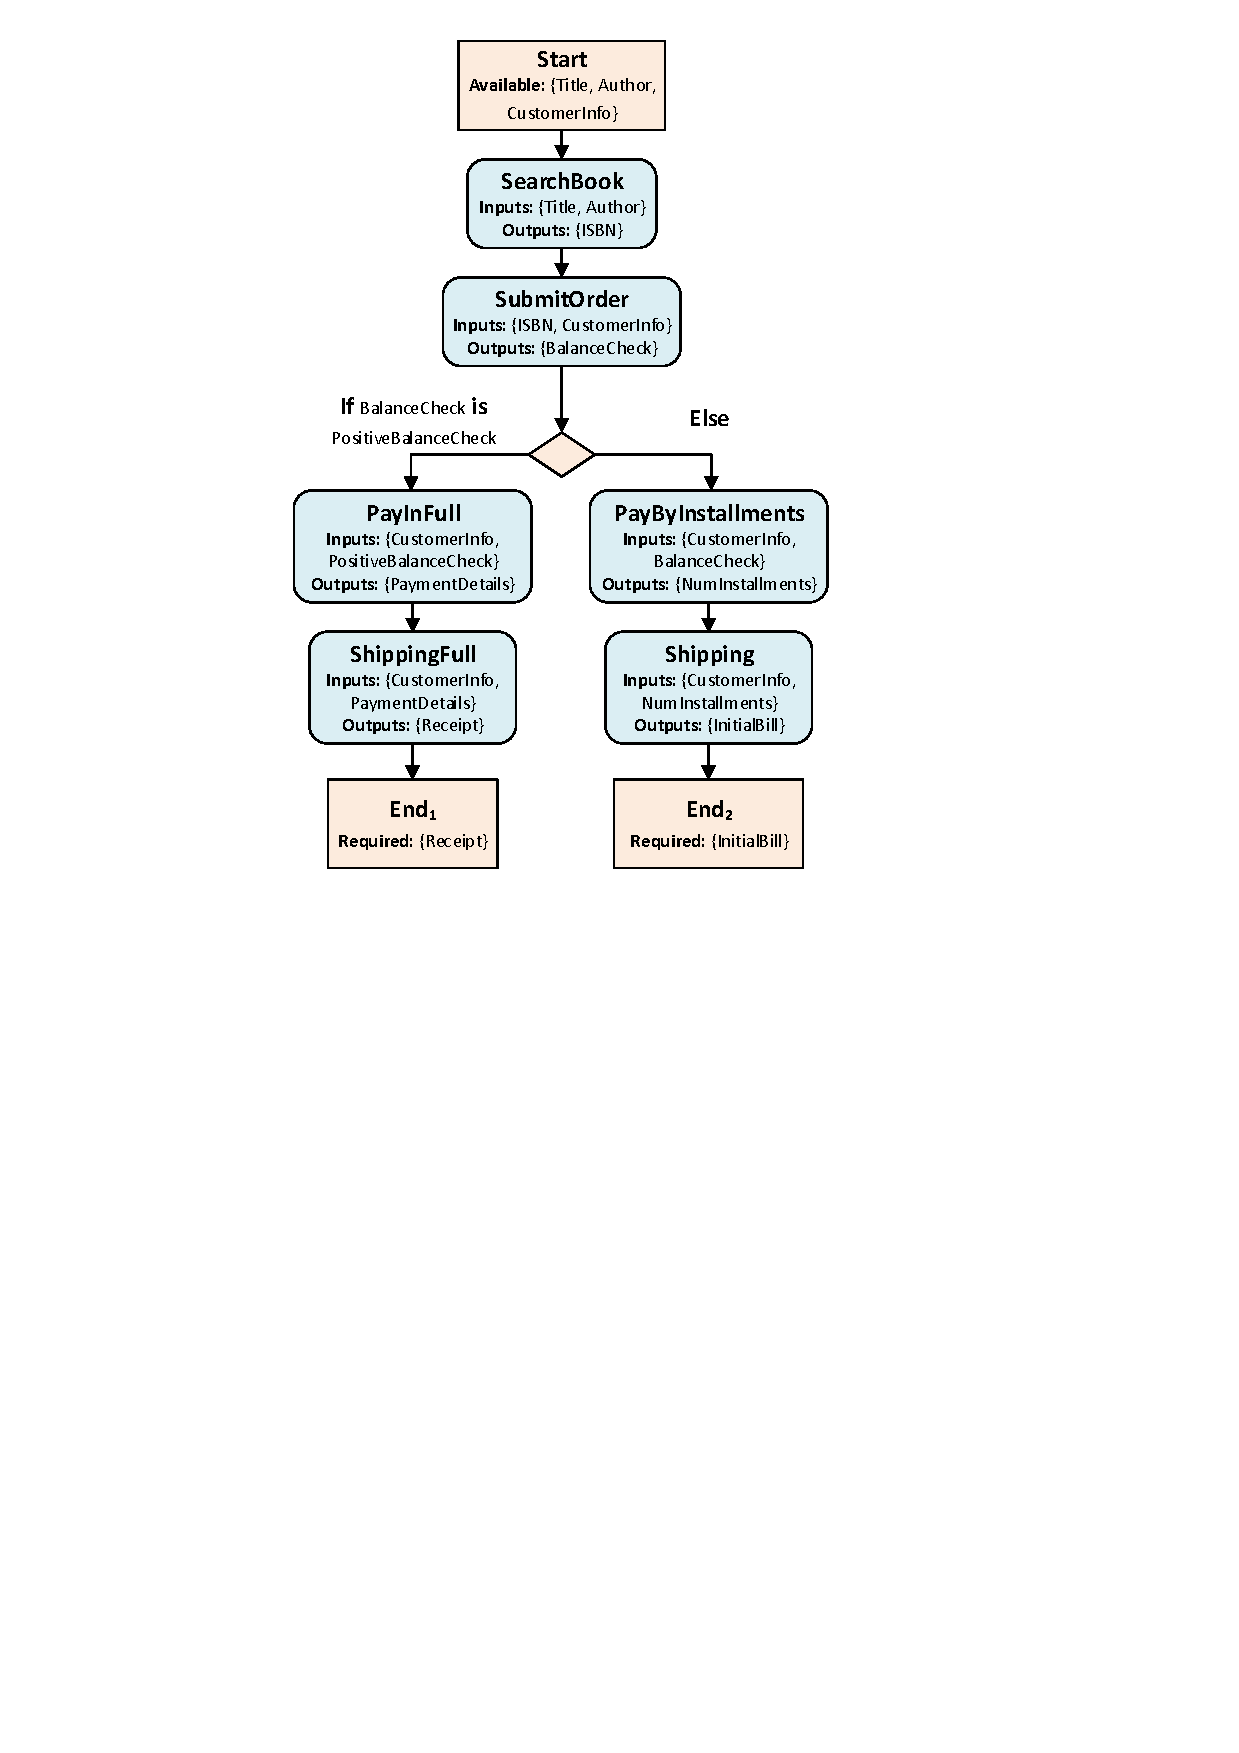
\includegraphics[width=7cm]{motivation.pdf}
}}
\caption{Example of composition requiring a branching constraint.}
\label{fig:motivation}
\end{figure}


\section{Background}\label{background}\label{constructs}

Languages for Web service composition, such as BPEL4WS \cite{wohed2003analysis}, offer constructs to describe how services interact to each other when assembled into a composite 
service in terms of input satisfaction and output production. However, in addition to these functional aspects, the non-functional attributes of each service (i.e. 
their quality) must also be considered when producing a composition. In this work, four QoS measures are taken into account \cite{jaeger2007qos,yu2013adaptive}: Time (\textit{T}), which indicates 
the 
execution time of a service between sending a request and receiving a response; Cost (\textit{C}), which is the financial cost associated with utilising the 
service; Availability (\textit{A}), which is the probability of a service being available when requested for execution, and Reliability (\textit{R}), which is 
the probability of a service responding appropriately when receiving a request. These attributes are associated with individual services, but can be calculated 
for a service composition according to the constructs used in it. The following constructs are employed in the proposed representation: 

\begin{itemize}
\item \textit{Sequence construct:} In a sequence construct services are executed sequentially, with the outputs of a service feeding the inputs of the next. 
This is depicted in Figure \ref{fig:sequence}. When calculating the overall QoS attributes for a sequence construct, the availability and probability values of all atomic
services are multiplied, while the time and cost are added.

\item \textit{Parallel construct:} In a parallel construct, services are executed in parallel with their inputs being independently satisfied and their outputs 
independently produced. This construct is shown in Figure \ref{fig:parallel}. The QoS attributes are calculated just as they are for the sequence construct, except for the 
time, which is considered to be that of the atomic service with the longest execution time.

\item \textit{Conditional construct:} In a conditional construct, only one of \textit{m} services will be executed depending on whether a given value condition is met. 
In this construct, the produced output is one of \textit{m} possible sets, as shown in Figure \ref{fig:conditional}. The likelihood of producing each of the \textit{m} sets is represented as
a probability value, with the probabilities for the sets adding up to 1. Therefore, the QoS attributes for the conditional construct are calculated using the
weighted sum of each quality attribute over all possible services, using the probabilities as the weights.

\begin{figure}
\centerline{
\fbox{
\begin{tabular}{p{0.9\linewidth}}
\space\hfill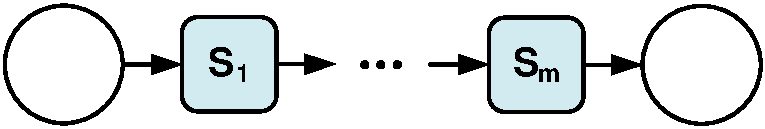
\includegraphics[width=2in]{sequence.pdf}\hfill\space\\[0.2cm]
$T=\frac{\sum\limits^m_{n=1}t_n}{m}$ \hfill $C=\frac{\sum\limits^m_{n=1}c_n}{m}$ \hfill
$A=\prod\limits^m_{n=1}a_n$ \hfill $R=\prod\limits^m_{n=1}r_n$
\end{tabular}}}
\caption{Sequence construct and calculation of its QoS properties
\cite{silva2014graph}.}
\label{fig:sequence}
\vspace{0.3cm}

\centerline{
\fbox{
\begin{tabular}{p{0.9\linewidth}}
\space\hfill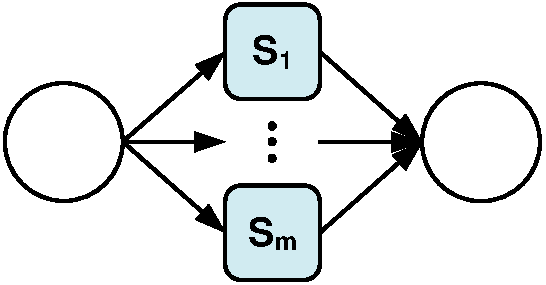
\includegraphics[width=1.4in]{parallel.pdf}\hfill\space\\[0.2cm]
\space\hfill$T=MAX\{t_n|n\in\{1,\ldots,m\}\}$\hfill\space\\[0.2cm]
$C=\frac{\sum\limits^m_{n=1}c_n}{m}$ \hfill $A=\prod\limits^m_{n=1}a_n$ \hfill
$R=\prod\limits^m_{n=1}r_n$
\end{tabular}}}
\caption{Parallel construct and calculation of its QoS properties
\cite{silva2014graph}.}
\label{fig:parallel}
\vspace{0.3cm}

\centerline{
\fbox{
\begin{tabular}{p{0.9\linewidth}}
\space\hfill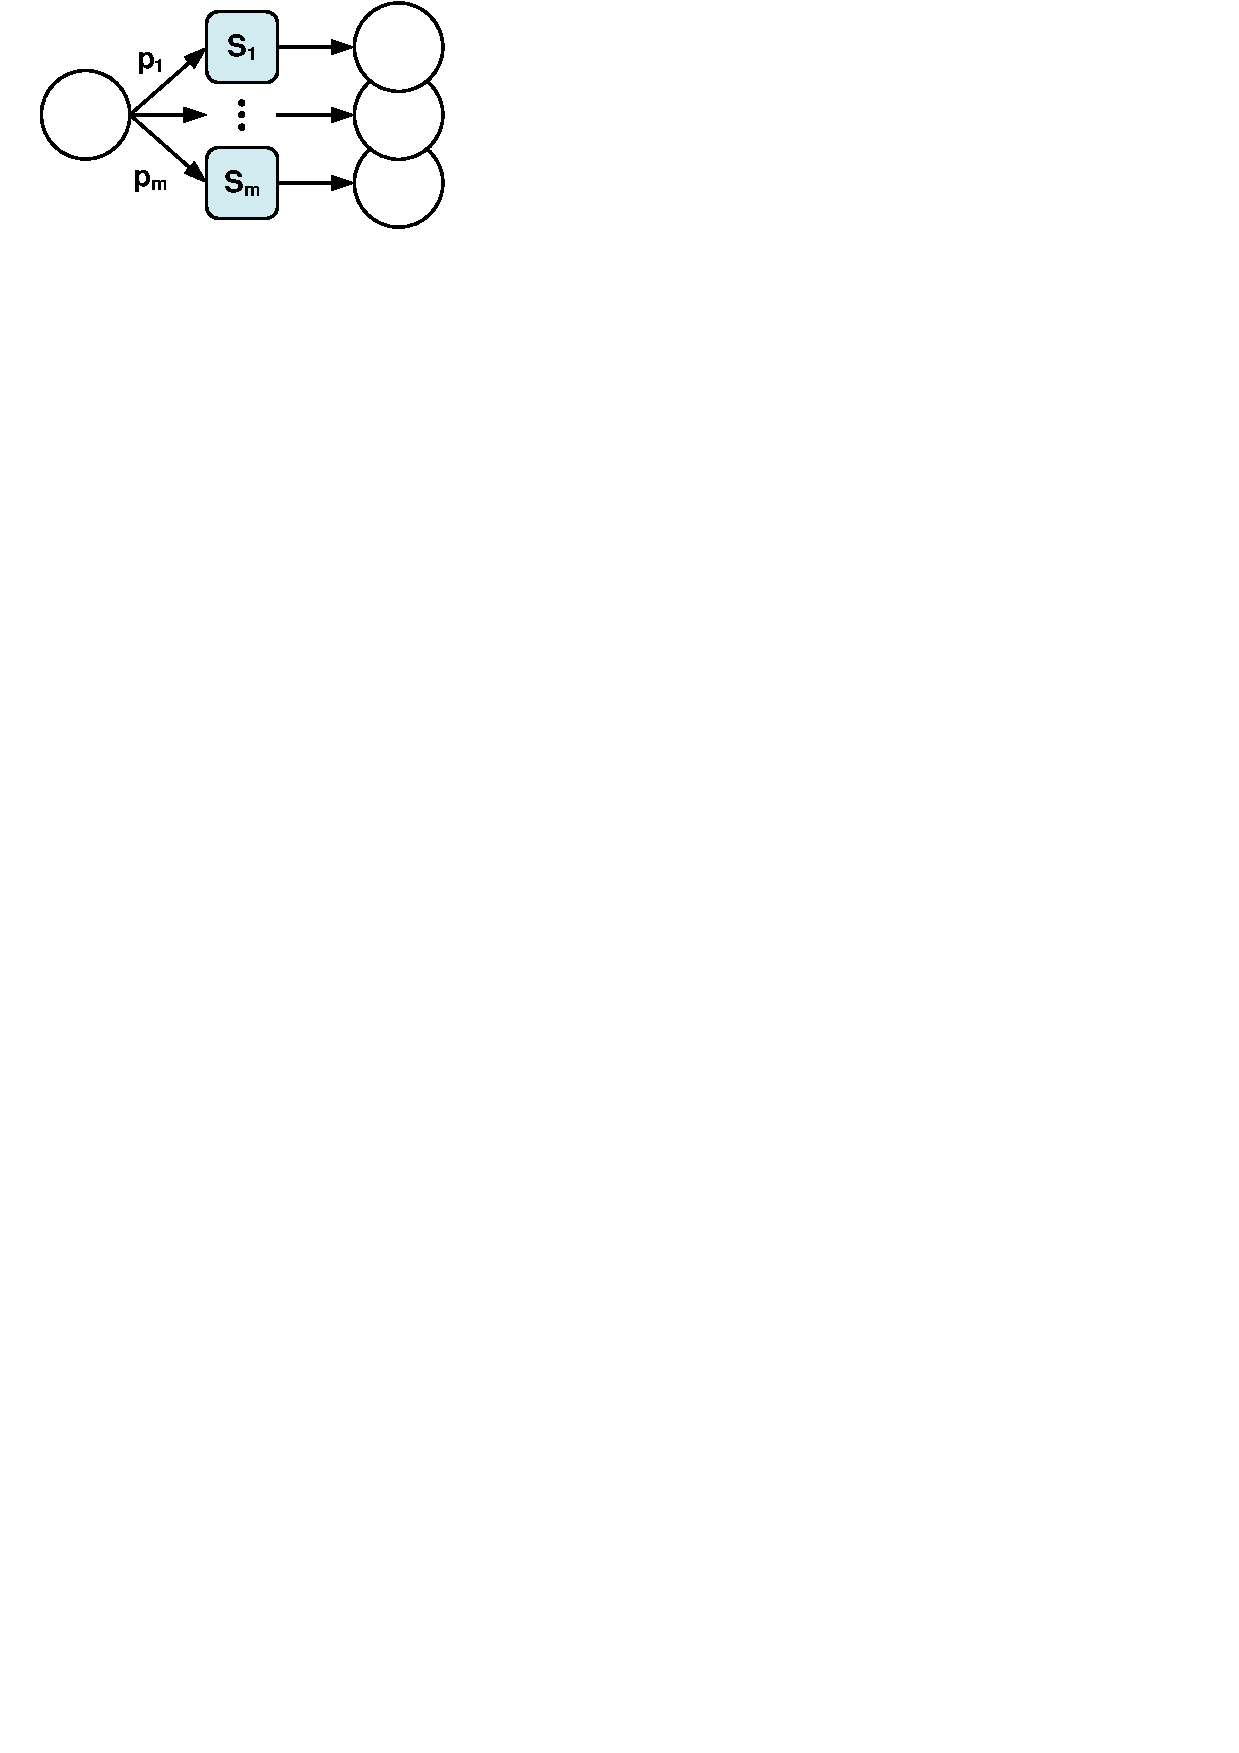
\includegraphics[width=1.4in]{conditional.pdf}\hfill\space\\[0.2cm]
$T=\sum\limits^m_{n=1}p_{n} t_{n}$ \hfill $C=\sum\limits^m_{n=1}p_{n} c_{n}$\hfill
$A=\sum\limits^m_{n=1}p_{n} a_{n}$\\
\space\hfill$R=\sum\limits^m_{n=1}p_{n} r_{n}$\hfill\space\\[0.2cm]
\end{tabular}}}
\caption{Conditional construct and calculation of its QoS properties.}
\label{fig:conditional}
\end{figure}

\end{itemize} 

\section{Proposed Approach}\label{approach}
The proposed approach employs Genetic Programming to evolve solutions according to their overall Quality of Service, meanwhile maintaining their functional 
correctness. In order to do so, a population initialisation algorithm similar to the one in \cite{wang2013genetic} is employed, and so are constrained mutation and crossover operations. However, the difference of the current approach in comparison to \cite{wang2013genetic} is that it also considers the case where a user requires a branching constraint to be met, like the one illustrated in Figure \ref{fig:motivation}. The presence of branching means that different values are produced by a service at runtime, and these concrete values are subtypes of a statically defined concept. For example, a service that statically outputs a \textit{fruit} concept may output the subtype \textit{banana} at runtime, and thus branching conditions may be defined based on the different kinds of fruits. The relationship between types is held by a taxonomy that encodes the inputs and outputs pertinent to the candidate atomic services employed in the composition. For simplicity, the implementation presented in this work handles branching with two options (if and else), so this scenario will be the focus throughout the following sections. In this work, a candidate solution for a composition is represented as a tree, where the non-terminal nodes represent the composition flow constructs (sequence, parallel, and conditional), and the terminal (leaf) nodes represent the atomic Web services included in the composition.

\subsection{Population Initialisation}\label{init}
As opposed to generating a composition candidate purely based on a set of available inputs and another of desired outputs, when handling branching constraints it is also necessary to consider a branching condition. Thus, a composition task with branching must include a set of available inputs, a condition of the is-a kind (e.g. if \textit{fruit} is a \textit{banana}), and two sets of outputs, one expected in case the condition is met and the other in case it is not. With this information it is possible to run the initialisation algorithm and create a composition candidate in graph format, later translated into a tree representation.

\begin{algorithm}
 \setlength\hsize{0.9\linewidth}
 \SetKwInOut{Input}{Input}\SetKwInOut{Output}{Output}
 \SetKwFunction{createGraph}{createGraph}\SetKwFunction{toTree}{toTree}
 \LinesNumbered
 \SetNlSty{}{}{:}
 \Input{$I$, $O_1$, $O_2$, $C$, $P$}
 \Output{candidate tree $T$}
 \eIf{$O_2 \neq \emptyset$}{
  $G_1 \leftarrow \createGraph(I \cup C.if, O_1)$\;
  $G_2 \leftarrow \createGraph(I \cup C.else, O_2)$\;
  $T_1 \leftarrow \toTree(G_1.input)$\;
  $T_2 \leftarrow \toTree(G_2.input)$\;
  $T_3 \leftarrow$ new $ConditionalNode$($C$)\;
  $T_3.leftChild \leftarrow T_1$\;
  $T_3.rightChild \leftarrow T_2$\;
  \eIf{$C \sqsubseteq I$}{
    $T_3.prob \leftarrow P$\;
    \KwRet $T_3$\;
  }{
    $G_4 \leftarrow \createGraph(I, C.else)$\;
    $T_4 \leftarrow \toTree(G_4.input)$\;
    $T_3.prob \leftarrow T_4.final.P$\;
    $T \leftarrow$ new $SequenceNode$()\;
    $T.leftChild \leftarrow T_4$\;
    $T.rightChild \leftarrow T_3$\;
    \KwRet $T$\;
  }
 }{
  $G \leftarrow \createGraph(I, O_1)$\;
  $T \leftarrow \toTree(G.input)$\;
  \KwRet $T$\;
 }
 \vspace{2mm}
 \caption{\footnotesize Generating a new candidate tree or a mutated subtree.}
\label{generation}
\end{algorithm}

Algorithm \ref{generation} is used to create a candidate which may incorporate a branching constraint, though it is also capable of handling unconditional tasks. It requires a
set of inputs $I$, an if-else condition $C$, two sets of outputs $O_1$ (for if-branch) and $O_2$ (for else-branch). The set of probabilities $P$ is only required for a specific case, explained below, and $C$ as well as $O_2$ are not required for tasks without branching. The intuition behind this algorithm is to assemble a candidate tree in parts. Firstly, if the task has in fact two sets of outputs and a condition $C$, then two sub-composition graphs $G_1$ and $G_2$ are generated to represent the if and the else branches, respectively. This generation is performed using the $createGraph$ algorithm proposed in \cite{wang2013genetic}. Subsequently, these graphs are translated to trees $T_1$ and $T_2$ using the $toTree$ procedure proposed in Algorithm \ref{toTree}, and included as children of a $ConditionalNode$ created for condition $C$ (the left child represent the if-branch, and the right child the else-branch).

Secondly, the algorithm verifies that the value used for condition $C$ can be met by using the set of inputs $I$. If it can, then the set of probabilities $P$ of each branch being executed is associated to the $ConditionalNode$ and the tree is returned (this assumes that the probabilities for obtaining a specific value for the if condition in $C$ are already known -- typically during mutation). If it cannot, then another sub-composition graph $G_4$ is generated and translated to $T_4$, creating the part of the composition that leads from the available inputs $I$ to the value used in condition $C$. In this case, the probability associated with each branch of the condition is extracted from the last service in $T_4$ (i.e. the service that produces the overall sub-composition output that satisfies the value used in condition $C$), and a $SequenceNode$ is created as the tree root to link this deterministic part of the composition ($T_4$) to the conditional part ($T_3$). Finally, if no condition $C$ and output set $O_2$ are provided, then the candidate is generated purely by using the $createGraph$ and $toTree$ algorithms. 

For reasons of brevity, the $toTree$ procedure shown in Algorithm \ref{toTree} for converting a graph representation of a composition to a tree representation is not explained in detail. Its general idea is to recursively traverse a graph, starting from the start ($input$) node and working towards the end ($output$) node. At each node, the number of outgoing edges determines whether to create a sequential or a parallel construct, and $toTree$ recurses on each of the destination nodes of these outgoing edges. A tree representation of a candidate solution has the terminal nodes as Web services and the non-terminal nodes as Sequence, Parallel, and Conditional constructs. A tree version of the example from Figure \ref{fig:motivation} is shown in Figure \ref{fig:tree}. It is important to note that after creating the candidate tree, it must be traversed one final time to determine the input values required to execute each node of the tree, and the output values produced by each node. This information is recorded within each node.

\begin{algorithm}
 \setlength\hsize{0.9\linewidth}
 \SetKwInOut{Input}{Input}\SetKwInOut{Output}{Output}
 \SetKwFunction{createParallelNode}{createParallelNode}\SetKwFunction{toTree}{toTree}
 \SetKwProg{Procedure}{Procedure}{}{}
 \LinesNumbered
 \SetNlSty{}{}{:}
 \Procedure{\toTree{}}{
 \Input{$N$}
 \Output{tree $T$}
 \uIf{$N$ is leaf}{
  \KwRet $N$\;
  }
  \uElseIf{$N = input$}{
    \eIf{$|N.to| = 1$}{
      $T \leftarrow \toTree(next.to[0])$\;
    }{
      $T \leftarrow \createParallelNode(N.to)$\;
    }
  }
  \uElse{
    $r$\;
    $children \leftarrow N.to - output$\;
    \eIf{$|children| = 1$}{
      $r \leftarrow \toTree(children[0])$\;
    }{
      $r \leftarrow \createParallelNode(children)$\;
    }
    $T \leftarrow$ new $SequenceNode$()\;
    $T.leftChild \leftarrow N$\;
    $T.rightChild \leftarrow r$\;
  }
  \KwRet $T$\;
  }
 \Procedure{\createParallelNode{}}{
 \Input{$children$}
 \Output{tree $T$}
 $T \leftarrow$ new $ParallelNode$()\;
 $subtrees \leftarrow \{\}$\;
 \ForEach{$c$ in $children$}{
    $S \leftarrow\toTree(c)$\;
    $subtrees \leftarrow subtrees \cup \{S\}$\;
 }
 $T.children \leftarrow subtrees$\;
 \KwRet $T$\;
 }
 \vspace{2mm}
 \caption{\footnotesize Converting graph into tree representation.}
\label{toTree}
\end{algorithm} 

\begin{figure}
\centerline{
\fbox{
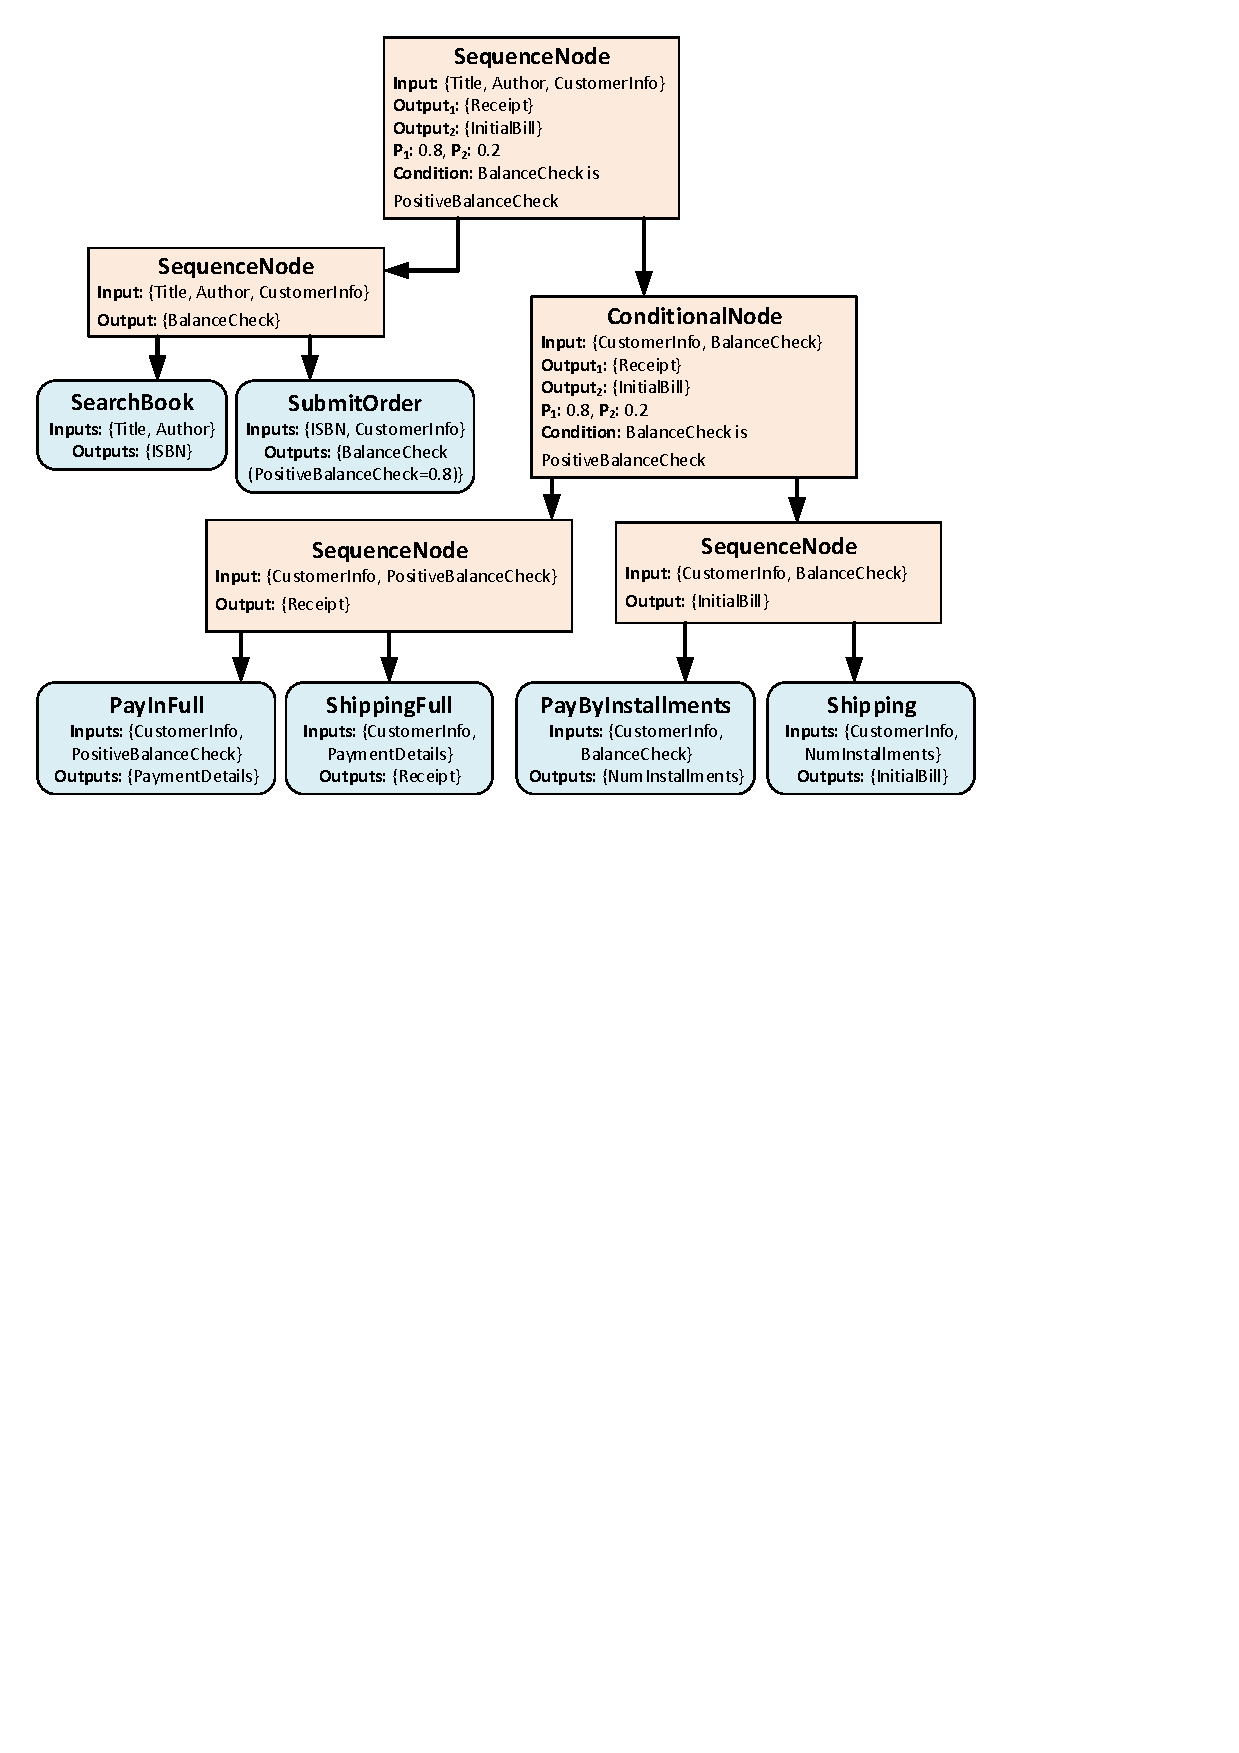
\includegraphics[width=8.4cm]{tree.pdf}
}}
\caption{Example of tree representation for Web service composition.}
\label{fig:tree}
\end{figure}

\subsection{Mutation and Crossover}\label{mutation}

The crossover operator employed in the evolutionary process swaps any two leaf nodes (i.e. Web services), one from each candidate, provided that these two leaves are functionally equivalent in terms of input and output values but represent different Web services. This particular crossover operation implementation was chosen because it provides an effective mechanism for performing Web service selection, whose objective is to identify the best service to perform a task out of a set of candidates providing the same functionality.
The mutation operator selects a node of the candidate tree at random, and using its input and output information produces a new subtree that may be structurally different yet provides the same functionality. The subtree is generated using Algorithm \ref{generation}, and is used to  replace the originally selected node in the candidate. In other words, the subtree of which the originally selected node was the root gives place to the newly generated subtree.


\subsection{Fitness Function}\label{fitness}

The fitness function is employed to measure the overall quality of a composition candidate. It does so by calculating the weighted sum of the four overall composition QoS attributes \cite{silva2014graph}, using the following function:

\begin{equation}
fitness_i = w_1(1 - A_i) + w_2(1 - R_i) + w_3T_i + w_4C_i
\end{equation}

\noindent where $\sum_{i=1}^{4} w_i = 1$
\\\\

This function produces values in the range [0, 1], with 0 representing the best possible quality and 1 the worst. The $A$, $R$, $T$, and $C$ values for each composition are calculated according to the formulae displayed in Figures \ref{fig:sequence}, \ref{fig:parallel}, and \ref{fig:conditional}. More specifically, the overall values are calculated starting from the tree leaves and working upwards towards the tree root. As the resulting fitness value must be between 0 and 1, the weights used in the function must add up to 1, and the QoS values must be normalised to the [0, 1] range. As availability ($A$) and reliability ($R$) are probability values, they already meet this requirement. The time and cost values for each Web service, on the other hand, are normalised by using the smallest ($Min$) and largest ($Max$) respective values in the dataset, according to the following functions:

\begin{equation}
T_i = \begin{cases}
     \frac{T_{orig} - T_{min}}{T_{max} - T_{min}}, & \text{ if $T_{max} - T_{min} \neq 0$}.\\
     1 & \text{ otherwise}.
    \end{cases}
\end{equation}

\begin{equation}
C_i = \begin{cases}
     \frac{C_{orig} - C_{min}}{C_{max} - C_{min}}, & \text{ if $C_{max} - C_{min} \neq 0$}.\\
     1 & \text{ otherwise}.
    \end{cases}
\end{equation}

Finally, $A$ and $R$ are offset by 1 in the fitness function. This is because $A$ and $R$ indicate the best qualities (i.e. the highest probabilities) with the highest possible values, whereas the fitness function indicates the best possible candidate quality with the lowest possible value (it is a minimising function).

\section{Experiments}\label{experiments}

Experiments were conducted to evaluate the performance of the proposed GP approach to service composition. One of the greatest hurdles in this process was the lack of datasets that supported the creation of compositions with branching. In order to enable the specification of branching conditions it is necessary to utilise a dataset that includes information about the different subtypes of outputs Web services may produce at runtime. For example, a Web service that outputs the result of a balance check to a customer's account (shown in Figure \ref{fig:motivation}) may return a positive balance check if the customer has enough funds to pay in full, or a negative balance check otherwise. Therefore, the service outputs the general \textit{balance check} type, but at runtime it may produce either the \textit{positive balance check} or the \textit{negative balance check} subtypes. By having this information, it is possible to create a composition whose execution is conditional on the runtime value of \textit{balance check}.

A consequence of considering the output possibilities of a service is that each possibility has an associated probability of being produced at runtime. For example, the probability of a balance check being positive could be 0.8, meaning that the probability of it being negative would be merely 0.2. These probabilities have been shown to be calculable by tracking the logged activities of a Web service, and to be a valuable tool in predicting execution patterns in a composition workflow \cite{clarke2014modelling}. In our work, output probabilities are used to calculate the quality of compositions that include a branch construct (as shown in Figure \ref{fig:tree}), where the branching condition is based on the possible runtime output values for a service. This means that the probability of a branch being chosen is dependent on the probabilities of a certain output being produced by the service whose value is used to satisfy the branching condition.

\subsection{Datasets}
The datasets to be used when testing this approach had to contain input and output information, including multiple output possibilities when appropriate, probability values for each of those possibilities, and QoS values for each Web service. As no datasets were found to provide all of these items, existing sets were extended to include all of the necessary information. The datasets in question are those used in \cite{wang2013genetic}, which are an augmented version of the 2008 Web Service Challenge (WSC2008) \cite{bansal2008wsc} that includes QoS attributes. Those datasets were chosen because they already provided an ontology of input and output value types that could be used to generate multiple output possibilities for a service, as well as quality values for optimisation.

The datasets were extended in two step. In the first step, new composition tasks were created for each dataset. As opposed to requiring the production of a single output set, the new tasks demand one of two sets to be produced depending on whether a branching condition is met, as exemplified by Figure \ref{fig:task}. Each of the tasks was manually ensured to be achievable. Additionally, new tasks that do not require branching were also created based on these branching tasks, for comparison purposes. These non-conditional tasks are similar to the branching ones, but they do not require conditions or multiple output sets (only the else-branch output set was kept). In the second step, to ensure that branching was in fact possible, all services in the dataset which produce the output types used in the branching condition were extended to produce two sets of outputs, one producing an instance of the specific concept (the \textit{if} condition) and another producing an instance of the general concept (the \textit{else} option). Finally, probabilities were randomly assigned to each output possibility, ensuring that the probabilities for all output sets of a same service would add up to 1.

\begin{figure}
\centerline{
\fbox{
 \lstset{basicstyle=\fontsize{7.5}{9.5}\ttfamily,columns=fullflexible}
 \lstinputlisting{task-example.xml}
 }}
 \caption{A task containing multiple output possibilities depending on a branching condition. The condition should be read as "if \textit{con1404081368} is of subtype \textit{con2027332959} at runtime, then the composition should produce \textit{if} outputs".}
 \label{fig:task}
\end{figure}


\subsection{Parameters}
The tests were carried out using a personal computer with an Intel Core i7-4770 CPU (3.4 GHz), and 8 GB RAM. 50 independent runs were conducted for each dataset, using both conditional (branching) and non-conditional (non-branching) tasks. For each run, a population of 20 candidates was used, and the evolutionary process produced exactly 50 generations. Crossover and mutation probabilities were set to 0.9 and 0.1, and elitism was set to 1 candidate. Tournament selection was used, with a tournament size of 7. As the candidate trees were already constrained by functional correctness mechanisms when initialising and evolving the population, no limit to the candidate tree depths was applied. All fitness function weights were set to 0.25, indicating that all QoS attributes are considered equally important by the composition requestor.

\subsection{Results and Discussion}

Experiment results are shown in Table \ref{results}, where the first column indicates the dataset used for execution and the number of services in it, the second and third columns contain the average fitness of the best solution and the average execution time in seconds for a run using the conditional task, and the fourth and fifth columns contain the average fitness and time for a run using the non-conditional task. All fitness and time values, including their standard deviation, are rounded to 3 decimal points of precision.

For both conditional and non-conditional tasks, the small standard deviation values for all fitness averages indicates that the algorithm converged to solutions with very similar fitnesses during the runs for each dataset. We hypothesise that these fitness averages are quite close to the global optimal solution for each task, though the exact optimal values are not known. Interestingly, the standard deviation for the average fitness of dataset 4's  conditional and non-conditional tasks are proportionately larger than those of any other sets, potentially indicating that the search space encoded in that set presents a more rugged topology than the others. In terms of execution time, an increase to the average occurs roughly proportionately to the increase in the total number of services in the dataset. The contrast between the average times for conditional and non-conditional tasks is stark, with non-conditional runs requiring significantly less time to execute for all datasets. While an increase in execution time was expected for conditional tasks due to the additional algorithmic steps required, it is interesting to find that using the branching construct had such an appreciable impact, even when some of the potential solutions were quite similar for the conditional and the non-conditional tasks (in some cases, a non-conditional solution could be made into a conditional one simply by adding one more service and a conditional node to the existing structure). The likely explanation for this is that the overhead of running the algorithm twice, once for each branch, causes the time increase regardless of the number of services contained within each branch. An informal investigation of the program's performance has shown that the algorithm for converting candidates from a graph to a tree representation, both for conditional and non-conditional tasks, presents an execution time bottleneck, indicating that improvements to its implementation could also be performed.


\begin{table}
\fontsize{6}{8}\selectfont
\centerline{
\def\arraystretch{1.5}
\begin{tabular}{c|c|c|c|c|}
\cline{2-5}
\textbf{}                                          & \multicolumn{2}{c|}{\textbf{Conditional}}      & \multicolumn{2}{c|}{\textbf{Non-conditional}}  \\ \hline
\multicolumn{1}{|c|}{\textbf{Set (size)}} & \textbf{Avg. fitness} & \textbf{Avg. time (s)} & \textbf{Avg. fitness} & \textbf{Avg. time (s)} \\ \hline
\multicolumn{1}{|c|}{1 (158)}                      & 0.601 $\pm$ 0.013     & 1.290 $\pm$ 0.100      & 0.588 $\pm$ 0.037     & 0.718 $\pm$ 0.079      \\ \hline
\multicolumn{1}{|c|}{2 (558)}                      & 0.712 $\pm$ 0.009     & 2.829 $\pm$ 0.250      & 0.694 $\pm$ 0.016     & 1.527 $\pm$ 0.194      \\ \hline
\multicolumn{1}{|c|}{3 (604)}                      & 0.631 $\pm$ 0.008     & 13.285 $\pm$ 1.229     & 0.788 $\pm$ 0.000     & 7.099 $\pm$ 0.906      \\ \hline
\multicolumn{1}{|c|}{4 (1041)}                     & 0.718 $\pm$ 0.048     & 6.146 $\pm$ 0.574      & 0.741 $\pm$ 0.429     & 3.568 $\pm$ 0.429      \\ \hline
\multicolumn{1}{|c|}{5 (1090)}                     & 0.698 $\pm$ 0.005     & 11.759 $\pm$ 0.948     & 0.688 $\pm$ 0.011     & 6.491 $\pm$ 0.743      \\ \hline
\multicolumn{1}{|c|}{6 (2198)}                     & 0.662 $\pm$ 0.017     & 92.392 $\pm$ 11.353    & 0.645 $\pm$ 0.024     & 52.308 $\pm$ 5.785     \\ \hline
\multicolumn{1}{|c|}{7 (4113)}                     & 0.578 $\pm$ 0.010     & 97.344 $\pm$ 13.705    & 0.688 $\pm$ 0.032     & 51.725 $\pm$ 4.260     \\ \hline
\multicolumn{1}{|c|}{8 (8119)}                     & 0.656 $\pm$ 0.005     & 326.387 $\pm$ 37.659   & 0.766 $\pm$ 0.002     & 186.896 $\pm$ 20.008   \\ \hline
\end{tabular}
}
\vspace{0.3cm}
\caption{Average fitness values and execution times for each dataset.}
\label{results}
\end{table}

A real candidate solution to the task shown earlier (Figure \ref{fig:task}) is depicted in Figure \ref{fig:solution}, demonstrating through an example that the proposed approach is capable of producing and optimising fully functional solutions. The root of the solution tree, which contains the input, both sets of outputs, and the branching condition, perfectly matches the information requested in the composition task, meaning that the task is fully satisfied. The root also displays a set of probabilities which shows that the likelihood of meeting the if-condition at runtime is 0.4 for this composition. The left child of the root node (i.e. \textit{serv1252722885}) produces outputs that lead to the branching condition, either producing an instance that matches the if-condition (\textit{inst572533116}) or an instance that matches the else-condition concept (\textit{inst2096765192}). Note that the other two outputs produced by this service do not vary. Finally, the branching condition concept is used as an input to one of the children of the conditional node (either \textit{serv763420204} or \textit{serv2014838942}) depending on its runtime value.

\begin{figure}
\centerline{
\fbox{
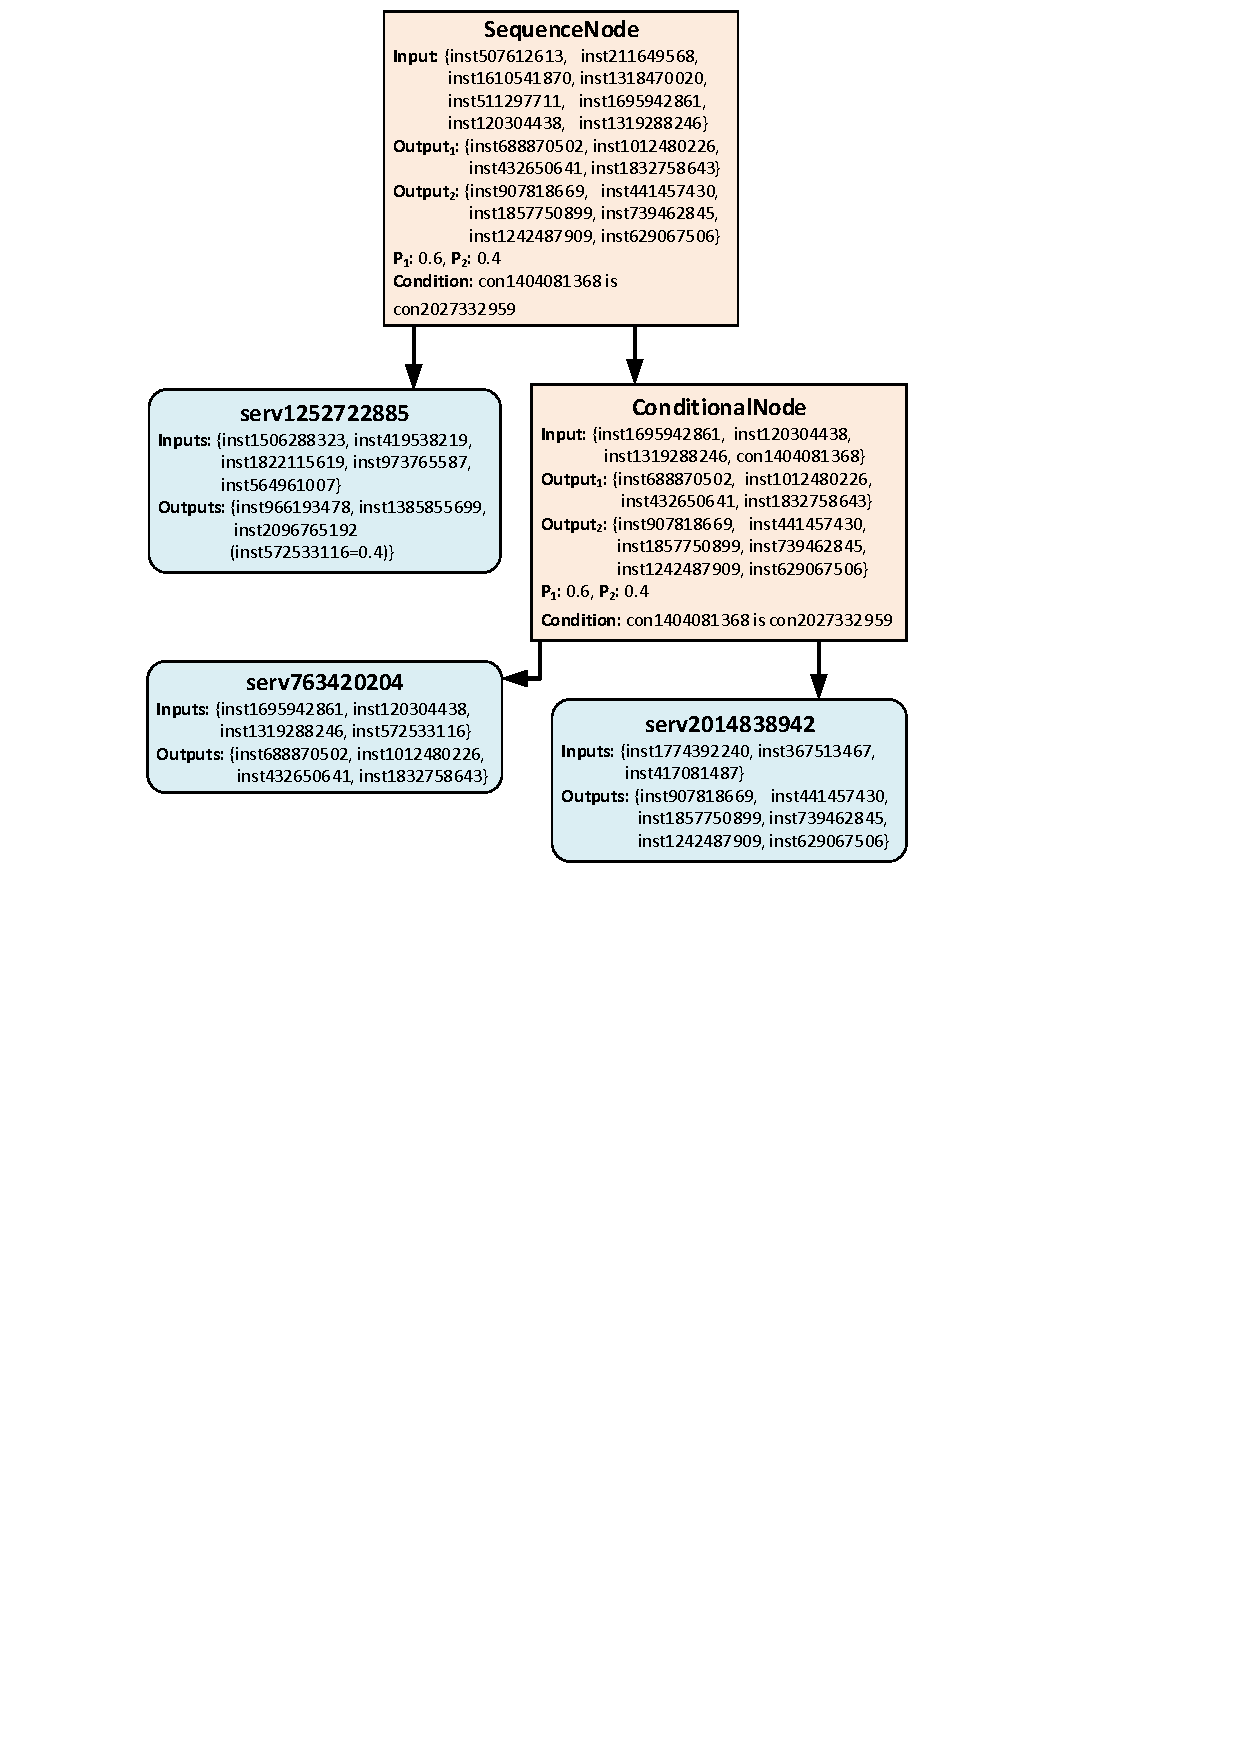
\includegraphics[width=8.4cm]{solution.pdf}
}}
\caption{A possible solution to the composition task shown earlier.}
\label{fig:solution}
\end{figure}

\section{Related Work}\label{related}

\subsection{AI Planning}
AI planning approaches to Web service composition ensure functional correctness by building a solution graph step by step. This solution graph may either be built to
enforce a set of user constraints, or it may be used to find an optimal solution in terms of QoS. However, no planning approaches in the literature have attempted to accomplish
both of these objectives simultaneously, which is a key difference from the work proposed in this paper. The approaches discussed below are representative of these two distinct research paths. For the constraints direction, it soon becomes evident that benchmarks to measure the effectiveness of solutions have not yet been established by researchers. This means that experiments in this area focus on demonstrating that approaches are capable of achieving compositions with that fulfil the required constraints, while comparisons between distinct approaches that consider branching are lacking. 

\cite{sohrabi2009web} presents an approach to include user preferences into the process of Web service composition. This is
accomplished by relying on a framework written in Golog, a language created for agent programming. Golog is used
to specify the particular attributes of generic workflows that represent commonly requested composition procedures
(an example of a generic workflow would be one that is dedicated to booking inter-city transportation).
The syntax of a logic-based language used to specify user preferences is described, allowing for
branching according to conditions, and for expressing preferences over alternative services.

In \cite{chen2014qos}, authors combine a planning algorithm and a graph search algorithm to achieve both QoS optimisation and functional correctness in Web service compositions. The
generic Graphplan algorithm first builds a representation of the search space as a planning graph, then finds a solution within this graph by traversing it backwards. This
standard planning approach is modified to use Dijkstra's algorithm when performing the backwards traversal, thus finding an optimised solution. The planning graph
is extended to include labels associated with each proposition (i.e. each intermediate action between two vertices), where each label contains a layer number and
associated execution costs. Dijkstra's algorithm is used to calculate the upcoming costs of each node in the graph. Then, a backtracking algorithm uses this
information to determine the optimal solution.

\subsection{EC Techniques}
EC techniques applied to Web service composition are primarily concerned with optimising the QoS of candidates, as well as producing functionally correct solutions. However, despite listing constructs with conditional constraints as a possibility, approaches in this area do not support tasks that include the specification of conditions, a gap that this work seeks to fill. The works discussed below represent merely one of the many facets in the vast area of EC-based service composition.

In \cite{wang2012survey}, an survey of the application of Genetic Algorithms (GA) to Web service composition is presented.
GAs are a popular choice for tackling combinatorial optimisation problems, and thus have been widely
applied to the problem of Web service composition. A common representation for atomic Web services uses integers,
meaning that each service is represented as an integer. The encoding scheme for a composition is commonly done 
as an array of integers, but some authors have attempted to use a matrix that includes semantic information. Researchers
also commonly investigate QoS representations, operators and fitness function variations to be applied to GA. An observed
problem with the GA technique is that it tends to prematurely converge to locally optimal solutions, thus preventing further 
exploration of possibilities.

\cite{wang2013genetic} employs GP to generate composition solutions that are functionally correct at all stages of execution, and are also optimised according to QoS attributes. A greedy algorithm is used to generate an initial population of functional candidates as graphs, which are then translated to a tree representation. Particular genetic operators are employed throughout the evolutionary process: the crossover operation ensures that the subtrees swapped between two candidates are functionally equivalent, thus preserving the correctness of the overall solution; the mutation operation replaces a randomly selected solution subtree with another one that is generated using the same algorithm employed for initialisation. Since the initialisation and genetic operators maintain functional correctness, the fitness function is only concerned with optimising solutions from a QoS perspective, which is done by calculating a weighted sum of the overall QoS attributes for the composition.

\subsection{Hybrid approaches}
Hybrid approaches combine elements of AI planning and optimisation techniques for solving the composition problem with functionally correct, optimised solutions. The hybrid approaches proposed in the literature are quite similar, relying on a directed acyclic graph as the base representation for a candidate solution, and then applying the optimisation techniques to this stucture. However, despite incorporating the use of planning techniques, these approaches do not include any discussion about the issue of producing solutions that satisfy user constraints or preferences. Another commonality between these works is that they require the use of SAWSDL-annotated datasets for testing, but these are not widely available to the research community. Therefore, authors developed their own datasets, and utilised each dataset's optimal task solution as the benchmark with which to evaluate the success of their implementation. More specifically, authors calculated the percentage of runs that culminated in the identification of the global optimum  as the recommended solution.

In \cite{pop2010immune}, an approach that combines AI planning and an immune-inspired algorithm is used to perform fully automated QoS-aware Web service composition, also considering
semantic properties. One significant contribution of this work is the proposal of an Enhanced Planning Graph (EPG), which extends the traditional planning graph structure
by incorporating semantic information such as ontology concepts. Given this data structure, the composition algorithm selects the best solution configuration from a set of candidates. A fitness function considering QoS values and semantic quality is used to judge the best solution, and a clonal selection approach is employed to perform the optimisation. Candidates cells (solutions) are cloned, matured (mutated by replacing services with others from the same cluster in the EPG) and the cell most suited to combating the invading organism (i.e. the best solution) is discovered.

\cite{pop2011hybrid} proposes the employment of the Firefly meta-heuristic technique for performing QoS-aware Web service composition, in conjunction with an AI planning strategy that uses an EPG as the basis for solutions. The firefly meta-heuristic is based on the behaviour of mating fireflies, which emit a flashing light to attract potential mates. Each artificial firefly investigates the search space, with each position representing a composition solution. The brightness of the firefly is represented by the fitness of the current solution (location) associated with it. Fireflies are attracted to others according to their brightness, which varies with distance. Finally, fireflies move towards the individuals they are attracted to, meaning that small modifications occur in the current solution. The fitness function represents the brightness of the solutions and takes into account the QoS attributes of the composition.

\section{Conclusion}\label{conclusion}
This paper presented a genetic programming approach to QoS-aware automated Web service composition. The novelty of this approach is that it addresses three composition dimensions simultaneously: the basic functional correctness of solutions (i.e. input-output matches), the use of branching constraints required by the user (i.e. complex functional correctness requirements), and the optimisation of solutions according to QoS attributes. The first two dimensions were handled by the utilisation of an algorithm to initialise and mutate solutions according to the required constraints, and the third dimension was handled by the utilisation of a fitness function that ranks solutions according to their overall QoS. No datasets with conditional tasks were available to test this approach, therefore the WSC2008 datasets were extended and used for this purpose. Results showed that the proposed approach was capable of identifying solutions that are fully functional and quality-optimised for all datasets, even though the average execution time was relatively high for the larger datasets. In particular, composition tasks that required the use of a branching construct necessitated significantly more time than tasks without branching.
While the approach proposed in this work is capable of handling two branches, it is not generalised to tackling an arbitrary number of branches and their associated conditions. Therefore, future work could extend this approach to flexibly handle scenarios that require several branches. The project could also be extended to handle more complex conditions, likely leading to the employment of a language to describe the constraints. Finally, modifications or extensions could be made aiming to improve the performance of the algorithms discussed in this paper.

\bibliographystyle{IEEEtran}
\bibliography{bibliography}

% that's all folks
\end{document}


